\documentclass[11pt,a4paper]{ctexart}
\usepackage[a4paper,margin=1.72cm]{geometry}
\usepackage{amsmath,amssymb,mathtools}
\usepackage{booktabs,tabularx,longtable,array,multirow}
\usepackage{enumitem}
\usepackage{tikz}
\usetikzlibrary{arrows.meta,positioning,shapes.geometric,fit,calc,matrix,decorations.pathreplacing}
\usepackage[most]{tcolorbox}
\usepackage{xcolor}
\usepackage{fancyhdr}
\usepackage{hyperref}
\usepackage{microtype}
\usepackage{listings}
\usepackage{pifont}
\usepackage{caption}
\newcolumntype{Y}{>{\raggedright\arraybackslash}X}
\setlength{\parindent}{2em}
\setcounter{secnumdepth}{0}
\setlength{\parskip}{0.30em}
\setlist[itemize]{itemsep=0.16em,topsep=0.26em}
\setlist[enumerate]{itemsep=0.16em,topsep=0.26em}
\hypersetup{colorlinks=true,linkcolor=blue!45!black,urlcolor=blue!50!black}

\definecolor{mainblue}{RGB}{45,86,140}
\definecolor{deepblue}{RGB}{30,62,102}
\definecolor{softblue}{RGB}{238,245,252}
\definecolor{softgreen}{RGB}{238,249,243}
\definecolor{softorange}{RGB}{253,246,233}
\definecolor{softred}{RGB}{253,239,239}
\definecolor{softgray}{RGB}{246,247,249}
\definecolor{deepgreen}{RGB}{35,105,75}
\definecolor{deeporange}{RGB}{165,98,22}
\definecolor{deepred}{RGB}{150,55,55}
\definecolor{purple}{RGB}{94,66,140}
\definecolor{softpurple}{RGB}{245,241,251}
\definecolor{teal}{RGB}{38,112,115}
\definecolor{softteal}{RGB}{238,248,248}
\definecolor{gold}{RGB}{156,120,28}
\definecolor{softgold}{RGB}{252,249,235}

\pagestyle{fancy}
\fancyhf{}
\lhead{408 OS 综合专题}
\rhead{内核状态机与跨子系统推演}
\cfoot{\thepage}
\renewcommand{\headrulewidth}{0.4pt}
\setlength{\headheight}{14pt}

\newtcolorbox{corebox}[1][]{colback=softblue,colframe=mainblue,title=#1,fonttitle=\bfseries,boxrule=0.8pt,arc=2mm}
\newtcolorbox{exam}[1][]{colback=softorange,colframe=deeporange,title=#1,fonttitle=\bfseries,boxrule=0.8pt,arc=2mm}
\newtcolorbox{warn}[1][]{colback=softred,colframe=deepred,title=#1,fonttitle=\bfseries,boxrule=0.8pt,arc=2mm}
\newtcolorbox{eng}[1][]{colback=softgreen,colframe=deepgreen,title=#1,fonttitle=\bfseries,boxrule=0.8pt,arc=2mm}
\newtcolorbox{method}[1][]{colback=softgray,colframe=black!45,title=#1,fonttitle=\bfseries,boxrule=0.6pt,arc=2mm}
\newtcolorbox{bridge}[1][]{colback=softpurple,colframe=purple,title=#1,fonttitle=\bfseries,boxrule=0.8pt,arc=2mm}
\newtcolorbox{statebox}[1][]{colback=softteal,colframe=teal,title=#1,fonttitle=\bfseries,boxrule=0.8pt,arc=2mm}
\newtcolorbox{history}[1][]{colback=softgold,colframe=gold,title=#1,fonttitle=\bfseries,boxrule=0.8pt,arc=2mm}

\newcommand{\kw}[1]{\textbf{#1}}
\newcommand{\code}[1]{\texttt{\detokenize{#1}}}
\newcommand{\arr}{\;\longrightarrow\;}
\newcommand{\yes}{\textcolor{deepgreen}{\ding{51}}}
\newcommand{\no}{\textcolor{deepred}{\ding{55}}}

% ---- Unified figure grammar: direct topology first ----
\tikzset{
  knode/.style={draw=mainblue,rounded corners=1.6mm,minimum width=2.55cm,minimum height=0.92cm,
    align=center,inner sep=3pt,font=\small,fill=softblue,line width=0.7pt},
  knodeg/.style={knode,draw=deepgreen,fill=softgreen},
  knodeo/.style={knode,draw=deeporange,fill=softorange},
  knodep/.style={knode,draw=purple,fill=softpurple},
  knodet/.style={knode,draw=teal,fill=softteal},
  knodegray/.style={knode,draw=black!45,fill=softgray},
  knodered/.style={knode,draw=deepred,fill=softred},
  persistent/.style={draw=deeporange,double,double distance=1pt,rounded corners=1.6mm,
    minimum width=2.55cm,minimum height=0.92cm,align=center,inner sep=3pt,font=\small,fill=softorange},
  mainflow/.style={-{Latex[length=2.2mm]},line width=0.9pt,draw=deepblue},
  relation/.style={-{Latex[length=1.8mm]},densely dashed,line width=0.8pt,draw=purple},
  optional/.style={-{Latex[length=1.8mm]},dotted,line width=0.9pt,draw=teal},
  danger/.style={-{Latex[length=1.8mm]},line width=0.9pt,draw=deepred},
  labelnote/.style={font=\scriptsize\bfseries,fill=white,inner sep=1.2pt,text=black!85,rounded corners=0.5pt}
}

\lstset{
  basicstyle=\ttfamily\small,
  columns=fullflexible,
  frame=single,
  rulecolor=\color{black!25},
  breaklines=true,
  showstringspaces=false,
  aboveskip=0.6em,
  belowskip=0.6em
}

\title{\vspace{-1.2cm}\textbf{操作系统综合专题：内核状态机与跨子系统推演}\\[0.35em]
\large 从对象、关系、队列到事件、机制、策略、不变量与成本的统一方法论}
\author{408 专题手册 · 操作系统总收束篇}
\date{}

\begin{document}
\maketitle

\begin{corebox}[本册只保留一个模型：不再把同一概念分散到多层重复讲]
前面的专题分别回答了进程、虚拟内存、并发、I/O、文件系统中的局部机制；本册只做一件事：建立一个\kw{不会重复定义同一概念}的统一内核模型，并用它推演跨专题问题。

唯一框架：
\[
\begin{aligned}
\boxed{\text{State：系统现在有什么}}\\[3pt]
\boxed{\text{Transition：系统怎样变化}}\\[3pt]
\boxed{\text{Evaluation：哪些变化合法、哪些更好}}
\end{aligned}
\]

其中：
\[
\boxed{S=(O,R,Q)}
\]
分别表示\kw{对象 Objects、关系 Relations、队列 Queues}；状态变化由\kw{事件 Event、机制 Mechanism、策略 Policy}共同决定；所有变化必须满足\kw{不变量 Invariants}，并承担一定\kw{成本 Cost}。
\end{corebox}

\begin{warn}[去重原则：每个元概念只有一个“正式住所”]
\begin{center}
\small
\begin{tabularx}{\linewidth}{>{\bfseries}p{0.25\linewidth} X X}
\toprule
元概念 & 唯一归属 & 不再重复出现为什么成立 \\
\midrule
Naming / Indirection & State 中的 Relations & 它描述“谁通过什么名字/映射指向谁”，不是独立运行规律 \\
Protection / Isolation & Evaluation / Invariants & 它回答“哪些状态/操作不允许出现”，不是第二套状态结构 \\
Mechanism / Policy & Transition & 机制定义可发生的转换，策略只在合法转换中选择 \\
Scarcity / Arbitration & Queue + Policy & 稀缺表现为请求进入队列；仲裁就是策略选谁获得资源 \\
Consistency / Recovery & Invariant + Repair & 一致性是不变量；恢复是故障后重新建立不变量的转换 \\
Fast / Slow Path & Cost Optimization & 它只回答“怎样把常见情况做便宜”，不再作为运行定律 \\
Event-driven Model & Transition 的驱动力 & Event 是状态变化的触发输入，本身不再另设一层 \\
Lifetime / Ownership & O/R 演化 + 生命周期约束 & 对象何时销毁取决于引用关系与生命周期不变量 \\
Caching / Laziness & Cost Optimization & 是利用局部性和推迟工作来降低成本的技术 \\
\bottomrule
\end{tabularx}
\end{center}
\end{warn}

\tableofcontents
\newpage

\section{第 0 章：删掉章节名以后，操作系统还剩下什么}

\subsection{操作系统不是五套机制的拼盘}
如果把“进程管理、内存管理、并发、I/O、文件系统”这些教材章节名全部删掉，内核仍然在持续做同一种工作：
\begin{enumerate}
  \item 维护一组对象以及对象之间的关系；
  \item 接收来自程序、硬件、时间和内部子系统的事件；
  \item 依据硬件机制和内核机制改变系统状态；
  \item 当存在多个合法选择时，根据策略决定下一步；
  \item 保证新的状态仍满足安全、隔离、进展、一致性与生命周期要求；
  \item 在正确性的约束下尽量降低延迟、空间、I/O、竞争和恢复成本。
\end{enumerate}

因此本册的总模型不是一句口号，而是一套可直接用于推题的形式化描述。

\subsection{统一状态转移模型}
设内核当前状态为
\[
S_t=(O_t,R_t,Q_t),
\]
其中：
\begin{itemize}
  \item $O_t$：当前存在的内核对象及其内部状态；
  \item $R_t$：对象之间的引用、映射、所有权与命名关系；
  \item $Q_t$：由于资源稀缺、等待条件或异步请求形成的队列。
\end{itemize}

某个事件 $E_t$ 到来以后，机制 $M$ 给出此时\kw{允许发生}的动作集合：
\[
\mathcal A_t=M(S_t,E_t).
\]
如果存在多个合法动作，策略 $\pi$ 选择其中一个：
\[
a_t=\pi(S_t,E_t,\mathcal A_t).
\]
随后状态转换：
\[
\boxed{S_{t+1}=T(S_t,E_t,a_t)}.
\]
但不是任何 $S_{t+1}$ 都允许存在，必须满足：
\[
\boxed{I(S_{t+1})=\text{true}},
\]
并在满足正确性的前提下优化成本：
\[
\boxed{\min C(S_t,E_t,a_t)}.
\]

\begin{corebox}[一句话总模型]
\[
\boxed{
\text{OS}=\text{State}+\text{Event}+\text{Allowed Transition}+\text{Policy}+\text{Invariant}+\text{Cost}
}
\]
进程、页表、锁、fd、inode、设备都只是 $O$ 中不同类型的对象；地址映射、fd 引用、路径解析都只是 $R$ 中不同类型的关系；run queue、wait queue、I/O queue 都只是 $Q$ 的不同实例。
\end{corebox}

\subsection{三维模型为什么不会重复}
\begin{center}
\small
\begin{tabularx}{\linewidth}{>{\bfseries}p{0.20\linewidth} X X}
\toprule
维度 & 唯一问题 & 典型关键词 \\
\midrule
State & \kw{现在有什么？彼此怎么连接？谁在等？} & object, reference, mapping, queue, owner, state \\
Transition & \kw{什么事件来了？允许怎么改？实际选哪种改法？} & event, mechanism, policy, wakeup, fault, interrupt \\
Evaluation & \kw{哪些状态绝不能出现？怎样更快/更省？} & protection, invariant, liveness, consistency, cache, fast path \\
\bottomrule
\end{tabularx}
\end{center}

这三维不存在“同一概念换名字再讲一遍”的必要：\kw{保护}永远是合法性约束；\kw{仲裁}永远是有队列时的策略选择；\kw{间接层}永远是对象关系的一种表示。

\newpage
\section{Part I：State——内核现在到底保存了什么}

\section{第 1 章：Objects——内核首先是对象管理器}

\subsection{对象的统一定义}
一个内核对象不是“一个结构体名字”，而是内核需要长期追踪的逻辑实体。任何对象都可以先用三元组理解：
\[
\boxed{Object=(Identity,\ State,\ Lifetime)}.
\]

\begin{center}
\scriptsize
\begin{tabularx}{\linewidth}{>{\bfseries}p{0.18\linewidth} >{\raggedright\arraybackslash}p{0.20\linewidth} Y Y}
\toprule
对象 & Identity & State & Lifetime 关键事件 \\
\midrule
Task/Thread & PID/TID/内核引用 & Running / Ready / Blocked；寄存器上下文 & create / exit / wait / reap \\
Address Space & mm/VMA 集合 & 映射、权限、驻留状态 & fork / exec / unmap / exit \\
Physical Page & PFN/页对象 & clean / dirty / referenced / pinned & alloc / reclaim / free \\
Open File & 内核 file object & offset、flags、引用计数 & open / dup / close \\
Inode & 文件系统对象身份 & size、mode、mapping、links & create / link / unlink / evict \\
Lock/Sync Object & 锁对象地址/句柄 & owner、waiters、计数 & init / acquire / release / destroy \\
Device/Request & device/request identity & pending / in-flight / done / error & submit / complete / retry \\
\bottomrule
\end{tabularx}
\end{center}

\begin{method}[跨专题第一问]
不要先问“这是哪一章的题”。先列出\kw{本题真正存在的对象}。一旦对象列错，后面的状态、引用、等待和生命周期一定会错。
\end{method}

\subsection{对象状态与对象身份必须分开}
一个对象可以改变状态，却仍然是同一个对象：
\[
Task:\ Running\arr Blocked\arr Ready.
\]
一个名字也可以改变，却不改变对象：
\[
\text{rename(pathA,pathB)}
\]
改变命名关系，但 inode 对象可以保持不变。

这就是为什么本册把\kw{Name}从 Object 中剥离：名字是引用入口，不是对象本身。

\section{第 2 章：Relations——Naming、Reference、Mapping 都只是“边”}

\subsection{统一关系图}
对象之间最重要的不是“层数”，而是\kw{边的语义}。典型关系如下：
\[
\boxed{Source\ Object/Name\xrightarrow{relation}Target\ Object}.
\]

\begin{center}
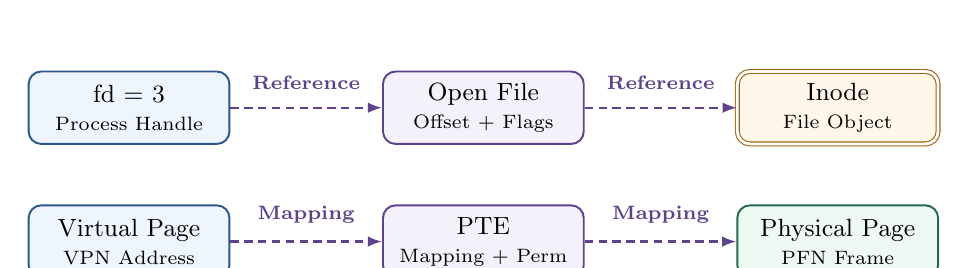
\begin{tikzpicture}[x=4.50cm,y=1.70cm]
  \node[knode] (fd) at (0,0) {fd = 3\\[-1pt]\scriptsize Process Handle};
  \node[knodep] (file) at (1,0) {Open File\\[-1pt]\scriptsize Offset + Flags};
  \node[persistent] (inode) at (2,0) {Inode\\[-1pt]\scriptsize File Object};
  \node[knode] (va) at (0,-1) {Virtual Page\\[-1pt]\scriptsize VPN Address};
  \node[knodep] (pte) at (1,-1) {PTE\\[-1pt]\scriptsize Mapping + Perm};
  \node[knodeg] (frame) at (2,-1) {Physical Page\\[-1pt]\scriptsize PFN Frame};
  \draw[relation] (fd) -- node[above=3pt,font=\scriptsize\bfseries,text=purple]{Reference} (file);
  \draw[relation] (file) -- node[above=3pt,font=\scriptsize\bfseries,text=purple]{Reference} (inode);
  \draw[relation] (va) -- node[above=3pt,font=\scriptsize\bfseries,text=purple]{Mapping} (pte);
  \draw[relation] (pte) -- node[above=3pt,font=\scriptsize\bfseries,text=purple]{Mapping} (frame);
\end{tikzpicture}
\end{center}

\subsection{Naming \& Indirection 的唯一位置}
\kw{Naming \& Indirection} 在本册中不再作为独立“哲学层”出现，它只回答 State 中的一个问题：

\begin{quote}
一个用户可见的名字、句柄或逻辑地址，通过哪些中间关系最终引用哪个对象？
\end{quote}

典型实例：
\[
\text{path}\arr\text{directory/dentry relation}\arr\text{inode},
\]
\[
\text{fd}\arr\text{open-file reference}\arr\text{file object},
\]
\[
\text{VPN}\arr\text{page-table mapping}\arr\text{PFN},
\]
\[
\text{file offset}\arr\text{block mapping}\arr\text{storage block}.
\]

\begin{corebox}[间接层真正买来的东西]
增加一层关系查找会增加成本，但换来：\kw{重定位、共享、隔离、重命名、稀疏表示、延迟绑定、权限检查、生命周期解耦}。

因此 Indirection 的本质不是“多查一张表”，而是：
\[
\boxed{\text{用一次额外查找换取对象与名字/位置/实现之间的解耦。}}
\]
\end{corebox}

\subsection{关系改变 ≠ 对象改变}
最经典例子是：
\[
\text{unlink(path)}.
\]
它首先删除的是：
\[
\text{Name}\dashrightarrow\text{inode}
\]
这条命名关系；如果仍存在：
\[
fd\dashrightarrow OpenFile\dashrightarrow inode,
\]
对象仍可继续使用。

因此所有生命周期题都应先画引用图，而不是背“删除文件”的口号。

\section{第 3 章：Queues——稀缺和等待在状态中的统一表示}

\subsection{为什么 Queue 属于 State，而不是“调度算法”}
队列描述的是\kw{当前有哪些请求正在等待某个条件或资源}。它本身是一部分系统状态，而不是策略。

\begin{center}
\scriptsize
\begin{tabularx}{\linewidth}{>{\bfseries}p{0.24\linewidth} Y Y}
\toprule
队列/等待结构 & 等待什么 & 谁/什么事件使其离开 \\
\midrule
Run Queue & CPU 时间 & scheduler dispatch \\
Lock Wait Queue & 锁/条件成立 & unlock / signal / wakeup \\
I/O Request Queue & 设备服务能力 & device dispatch / completion \\
Pipe Waiters & buffer 非空/非满 & peer read / write \\
Reclaim/Writeback & 内存/脏页压力释放 & reclaim / writeback completion \\
\bottomrule
\end{tabularx}
\end{center}

\subsection{Scarcity 不再单独成章}
所谓“有限资源下的仲裁”可以严格拆成两个已经存在的元素：
\[
\boxed{\text{Scarcity}\Rightarrow\text{Queue state appears}}
\]
和
\[
\boxed{\text{Arbitration}\Rightarrow\text{Policy selects a waiter/request}}.
\]

所以“Scarcity/Arbitration”不需要再做一条 Law。它是\kw{State 的 Queue + Transition 的 Policy}组合出来的现象。

\begin{statebox}[需求大于供给时的通用状态变化]
\[
\text{Request}\arr
\begin{cases}
\text{Grant}, & Capacity>0,\\
\text{Enqueue/Block/Reject}, & Capacity=0.
\end{cases}
\]
资源释放后再由策略决定：
\[
\text{Release}\arr\text{Choose Waiter}\arr\text{Wake/Grant}.
\]
\end{statebox}

\section{第 4 章：Lifetime——它不是第四种结构，而是对象与关系随时间的变化}

生命周期不需要与 Objects/Relations/Queues 并列成第四种 State 元素。它本质上是：
\begin{itemize}
  \item 对象何时加入或移出 $O$；
  \item 引用边何时加入或移出 $R$；
  \item 哪些生命周期不变量必须始终成立。
\end{itemize}

典型模式：
\[
\boxed{
Create\arr AddReference\arr Use\arr DropReference\arr Destroy
}
\]
但 Destroy 的条件不是“调用了 delete/close/free”，而是某个生命周期不变量成立，例如：
\[
\text{No reachable/open reference}\land\text{object no longer named/owned}.
\]

\begin{warn}[高频错误]
\kw{逻辑删除不等于立即销毁}。\code{unlink()}、\code{close()}、进程退出、page unmap 都可能只删除某一类关系；对象能否真正回收，要看剩余引用、所有权和子系统自己的生命周期规则。
\end{warn}

\newpage
\section{Part II：Transition——内核状态到底怎样变化}

\section{第 5 章：Event——状态变化的触发输入}

\subsection{内核是“事件驱动”的准确含义}
本册只把 Event 定义为：\kw{触发内核重新评估并可能改变状态的输入}。典型来源：
\begin{itemize}
  \item 程序主动：syscall、lock/unlock、exit；
  \item 当前指令同步产生：page fault、protection fault、illegal instruction；
  \item 硬件异步产生：timer、I/O completion interrupt；
  \item 内核内部产生：memory pressure、writeback threshold、timeout、wakeup；
  \item 故障产生：process crash、system crash、I/O error。
\end{itemize}

因此“事件驱动”不再另外成为一条 Law，它就是 Transition 的输入 $E_t$。

\begin{method}[事件识别法]
综合题中先圈出每一个真正改变状态的事件。例如：\code{read()} 调用、page-cache miss、进程睡眠、DMA completion、interrupt、wakeup、scheduler dispatch。不要把“执行了一段代码”笼统看成一个事件。
\end{method}

\section{第 6 章：Mechanism——定义“允许怎么变”}

机制回答：\kw{系统具备哪些受控状态转换能力？}

\begin{center}
\scriptsize
\begin{tabularx}{\linewidth}{>{\bfseries}p{0.24\linewidth} Y Y}
\toprule
机制 & 它允许的状态变化 & 它不负责决定什么 \\
\midrule
Trap/System-call entry & User execution $\to$ Kernel execution & 具体服务策略 \\
Context Switch & CPU context A $\to$ B & 下一次选 B 还是 C \\
Page Fault Handler & nonresident / permission fault $\to$ repair or reject & victim / allocation policy \\
Atomic RMW + Sleep/Wakeup & lock state / waiter state 可原子改变 & 谁应该先拿锁的公平策略 \\
Block I/O + DMA & request 可提交并异步完成 & 多请求先服务谁 \\
Journal/Replay & 多步持久更新可记录、提交、恢复 & 哪些高层操作何时触发持久化 \\
\bottomrule
\end{tabularx}
\end{center}

\section{第 7 章：Policy——只在“存在选择”时出现}

策略不是所有状态转换都需要。只有当机制给出了多个合法候选动作时，Policy 才有意义：
\[
\boxed{a_t=\pi(S_t,E_t,\mathcal A_t)}.
\]

典型：
\begin{itemize}
  \item scheduler：多个 Ready task 选谁；
  \item page replacement：多个可回收页选谁；
  \item I/O scheduling：多个 pending request 先发谁；
  \item lock fairness：多个 waiter 怎样排序；
  \item allocation：多个可用 frame/block/extent 选哪个。
\end{itemize}

\begin{corebox}[Mechanism / Policy 的边界]
\[
\boxed{Mechanism=\text{定义合法动作集合}}
\]
\[
\boxed{Policy=\text{从合法动作集合中选择}}
\]
如果只有一个合法动作，就没有策略问题；如果连动作都做不到，说明缺的是机制，不是策略。
\end{corebox}

\subsection{为什么这能消除“Law 3 vs Loop 2”的重复}
“有限资源下的仲裁”现在不再是第三套理论：
\begin{enumerate}
  \item State 中已经存在一个 Queue；
  \item Event 表示资源释放或请求到达；
  \item Mechanism 提供 enqueue/dequeue/block/wakeup 能力；
  \item Policy 决定从 Queue 中选谁；
  \item Invariant 检查不能重复授予、不能越权；
  \item Cost 再考虑公平性、等待时间和吞吐。
\end{enumerate}
因此没有必要再定义一个独立“Resource Arbitration Loop”。

\newpage
\section{Part III：Evaluation——什么叫“正确”，什么叫“更好”}

\section{第 8 章：Invariants——保护、一致性、进展都属于合法性约束}

\subsection{不变量的统一定义}
状态转换以后必须满足：
\[
\boxed{I(S_{t+1})=\text{true}}.
\]
所谓 Protection、Isolation、Atomicity、Consistency 并不是四套独立架构，它们都是\kw{对合法状态/合法转换的不同约束}。

\subsection{五类常见不变量}
\begin{center}
\scriptsize
\begin{tabularx}{\linewidth}{>{\bfseries}p{0.25\linewidth} Y Y}
\toprule
不变量类型 & 核心问题 & 典型例子 \\
\midrule
Safety & 什么绝不能发生？ & 同一独占资源不能同时授予两个 owner \\
Protection/Isolation & 谁能对哪个对象做什么？ & User 不能写 kernel page；fd 权限必须合法 \\
Progress/Liveness & 合法请求是否最终可能继续？ & 无死锁、无永久丢失唤醒；公平性视策略而定 \\
Structural Consistency & 对象/关系是否自洽？ & inode / block bitmap、引用计数、队列状态一致 \\
Persistence/Crash Consistency & 故障后能否恢复到合法持久状态？ & journal commit / replay 后 metadata 一致 \\
\bottomrule
\end{tabularx}
\end{center}

\begin{corebox}[Protection 的唯一住所]
保护在本册不再既当“OS 职责”又当“运行 Law”重复出现。统一写成约束：
\[
\boxed{Allowed(Subject,Operation,Object,Authority)}.
\]
任何状态转换只要违反这个谓词，就必须被硬件或内核拒绝、陷入、返回错误或终止。
\end{corebox}

\subsection{并发一致性与崩溃一致性的统一}
二者共同研究：\kw{一个逻辑操作被部分执行时，非法中间状态会不会暴露或永久留下。}

并发：
\[
A\arr B\arr C
\]
可能变成：
\[
A\arr\boxed{Interleaving}\arr B\arr C.
\]
崩溃：
\[
W_1\arr W_2\arr W_3
\]
可能变成：
\[
W_1\arr W_2\arr\boxed{Crash}.
\]

二者的共同目标都是：
\[
\boxed{\text{让外部可观察状态始终满足关键不变量，或能恢复到满足不变量的状态。}}
\]
手段不同：并发主要使用原子操作、锁、条件同步和有序提交；持久化主要使用 write ordering、journal/WAL、commit、replay、repair。

\section{第 9 章：Cost——性能原则只放在这一层}

\subsection{统一成本函数}
正确状态不止一个，因此还要关心：
\[
\boxed{\begin{aligned}
C={}&Latency+CPU+Space+MemoryTraffic\\
   &+IO+Contention+FairnessPenalty+RecoveryCost.
\end{aligned}}
\]
不同机制优化的是不同项，不能把“更快”当作单一目标。

\subsection{Fast / Slow Path 的唯一位置}
快慢路径不再是运行 Law，而是\kw{成本优化模式}：
\[
\boxed{CommonCase\rightarrow CheapFastPath}
\]
\[
\boxed{Miss/Conflict/Pressure\rightarrow RareComplexSlowPath}.
\]

\begin{center}
\small
\begin{tabularx}{\linewidth}{>{\bfseries}p{0.18\linewidth} X X}
\toprule
子系统 & Fast Path & Slow Path \\
\midrule
Virtual Memory & TLB hit / resident mapping & page-table walk / page fault / I/O \\
File System & dentry/page-cache hit & path miss / block mapping / storage I/O \\
Lock & uncontended atomic acquire & contention $\to$ wait queue / scheduler \\
I/O & buffered/cache hit / async device work & queueing / retry / error / wakeup \\
Process & direct user execution & syscall/exception/interrupt enters kernel \\
\bottomrule
\end{tabularx}
\end{center}

\subsection{Locality、Caching、Laziness、Batching 不是新“原则层”}
这些都只是降低 $C$ 的策略/技术：
\begin{itemize}
  \item \kw{Locality}：预测近期再次访问或访问邻近对象；
  \item \kw{Caching}：保存慢对象的快速副本；
  \item \kw{Laziness}：把工作推迟到真正需要时，如 demand paging、COW、delayed allocation；
  \item \kw{Batching}：把多个小动作合并，摊薄固定开销，如 writeback、I/O merging；
  \item \kw{Speculation/Prefetch}：提前做可能需要的工作，换取平均延迟下降。
\end{itemize}

\begin{warn}[优化不能破坏不变量]
所有性能机制必须服从：
\[
\boxed{\text{Correctness first, optimization second}.}
\]
COW 可以延迟复制，但不能破坏进程隔离；writeback 可以延迟持久化，但必须明确 durability 边界；lock fast path 可以省掉调度，但不能破坏互斥。
\end{warn}

\newpage
\section{Part IV：从模型到题目——只保留“轨迹模板”，不再创造新理论层}

\section{第 10 章：五种常见轨迹模板}

\begin{corebox}[定位说明]
下面五种不是新的 Laws、Loops 或 Principles。它们只是把前面的唯一模型投影到时间轴上，帮助做题时识别状态变化的常见形状。每一种都必须仍然回填 $O,R,Q,E,M,\pi,I,C$。
\end{corebox}

\subsection{轨迹 A：Resolve——名字/句柄/逻辑地址解析}
\[
\boxed{Name/Handle\arr RelationLookup\arr Object}
\]
例如：
\[
fd\arr OpenFile,
\qquad
VPN\arr PTE\arr Frame,
\qquad
Path\arr Dentry/Inode.
\]
这类题首先画 $R$，一般不涉及 Queue；若查找 miss/fault，再进入其他轨迹。

\subsection{轨迹 B：Wait / Wake——条件暂不满足}
\[
\boxed{Running\arr Check\arr Block/Enqueue\arr Event\arr Wake\arr Ready}
\]
例如锁竞争、阻塞 I/O、pipe empty/full、条件变量。核心状态是 $Q$ 和 task state；核心转换机制是 atomic sleep/wakeup；策略只在多个 waiter 中选择时出现。

\subsection{轨迹 C：Fault / Repair / Retry——映射或条件暂时不能满足}
\[
\boxed{Attempt\arr Fault/Miss\arr KernelRepair\arr UpdateState\arr Retry}
\]
典型：page fault、COW、file-backed mmap 首次访问。注意这不是“Mapping Loop”新理论，只是某次 Transition 的时间结构。

\subsection{轨迹 D：Pressure / Reclaim——需求超过容量}
\[
\boxed{Demand>Capacity\arr Pressure\arr SelectVictim\arr Reclaim/Writeback\arr Retry}
\]
这里的 SelectVictim 才是 Policy；reclaim/writeback 是 Mechanism；不能把整个过程笼统叫“页面置换算法”。

\subsection{轨迹 E：Modify / Commit / Recover——持久状态的多步更新}
\[
\boxed{Modify\arr Dirty/Pending\arr Commit\arr Stable}
\]
若故障：
\[
\boxed{Crash\arr InspectLog/Metadata\arr Replay/Repair\arr ConsistentState}.
\]
它用于区分“内存可见”“系统调用返回”“设备完成”“真正持久”这些不同状态。

\section{第 11 章：五大子系统在唯一模型中的投影}

\begin{center}
\scriptsize
\renewcommand{\arraystretch}{1.18}
\begin{tabularx}{\linewidth}{>{\bfseries}p{0.18\linewidth} Y Y Y}
\toprule
子系统 & Objects & Relations & Queues \\
\midrule
Process/Sched & task / thread & task$\to$mm/files & run / wait queue \\
VM & VMA / PTE / page & VA$\to$PTE$\to$frame & reclaim / writeback wait \\
Concurrency & lock / semaphore / waiter & owner / wait relation & lock / CV wait queue \\
I/O & device / request / buffer & request$\to$device & request / completion queue \\
File System & fd / file / inode / dentry & path / fd / offset mappings & writeback / cache-related waits \\
\bottomrule
\end{tabularx}
\end{center}

\begin{center}
\scriptsize
\renewcommand{\arraystretch}{1.18}
\begin{tabularx}{\linewidth}{>{\bfseries}p{0.18\linewidth} Y Y Y}
\toprule
子系统 & Events & Mechanism / Policy & Invariant / Cost \\
\midrule
Process/Sched & timer / syscall / exit & switch, block, wake / scheduling & execution correctness / response, fairness \\
VM & fault / pressure / unmap & map, fault, reclaim / replacement & isolation / miss, I/O, space \\
Concurrency & lock / unlock / signal & atomic + sleep/wake / fairness & mutual exclusion, order / contention \\
I/O & submit / interrupt / error & DMA, interrupt, driver / request order & request correctness / latency, BW, CPU \\
File System & open / read / write / unlink / crash & VFS, block map, journal / allocation & namespace, crash consistency / lookup, durability \\
\bottomrule
\end{tabularx}
\end{center}

\begin{bridge}[看矩阵的方法]
不要横着背整行。综合题应当\kw{竖着读一列，再跨列跟踪同一个事件}。例如一个 blocking read 会先修改 Process 列的 task state，再进入 File System 列解析对象，再进入 I/O 列提交请求，完成后又回到 Process 列 wakeup。
\end{bridge}

\newpage
\section{Part V：九大跨专题生命周期——同一套八问反复使用}

\section{第 12 章：统一“八槽分析表”}
任何跨专题母题，都只填写下面八个槽位：
\begin{enumerate}
  \item \kw{Objects}：涉及哪些对象？
  \item \kw{Relations}：谁指向谁、映射到谁？
  \item \kw{Queues}：谁在等什么？
  \item \kw{Event}：当前真正发生了什么触发事件？
  \item \kw{Mechanism}：系统用什么能力改变状态？
  \item \kw{Policy}：哪里存在“选谁/选哪个”的选择？没有就写“无”。
  \item \kw{Invariant}：什么绝不能被破坏？
  \item \kw{Cost}：主要成本在哪里？有没有 fast/slow path？
\end{enumerate}

\begin{method}[为什么只用八槽]
八槽与统一模型一一对应，不增加任何新分类。综合题的复杂度只来自\kw{对象多、事件多、跨多个子系统连续变化}，而不是需要额外学习另一套“综合理论”。
\end{method}

\section{第 13 章：母题一——程序从 fork 到 exec、运行、exit、wait}

\subsection{核心轨迹}
\[
\begin{aligned}
Parent&\xrightarrow{fork}Parent+Child\\
&\xrightarrow{exec}Child(NewAddressSpace)\\
&\xrightarrow{run/syscall/fault}RunningSystem\\
&\xrightarrow{exit}Zombie/ExitState\xrightarrow{wait}Reaped.
\end{aligned}
\]

\begin{center}
\small
\begin{tabularx}{\linewidth}{>{\bfseries}p{0.18\linewidth} X}
\toprule
槽位 & 本题关键内容 \\
\midrule
Objects & parent task、child task、address space、page tables、open files \\
Relations & child 初始继承/共享部分资源关系；exec 替换程序映像；fd 关系通常按规则保留 \\
Queues & child/parent 进入 run queue；wait 时 parent 可能进入 wait queue \\
Events & fork、exec、timer、fault、exit、wait \\
Mechanism & task create、COW、context switch、address-space replace、wake/reap \\
Policy & scheduler 选择谁运行 \\
Invariant & 地址空间隔离；父子资源引用合法；退出状态不被过早释放 \\
Cost & COW 减少 fork 初始复制；fault 把复制成本推迟到写入 slow path \\
\bottomrule
\end{tabularx}
\end{center}

\section{第 14 章：母题二——一次 blocking read(fd,buf,n)}

\subsection{四条信息同时追踪}
综合版不再只画一条调用栈，而同时追踪：\kw{Control、Task State、Data、Reference}。

\begin{center}
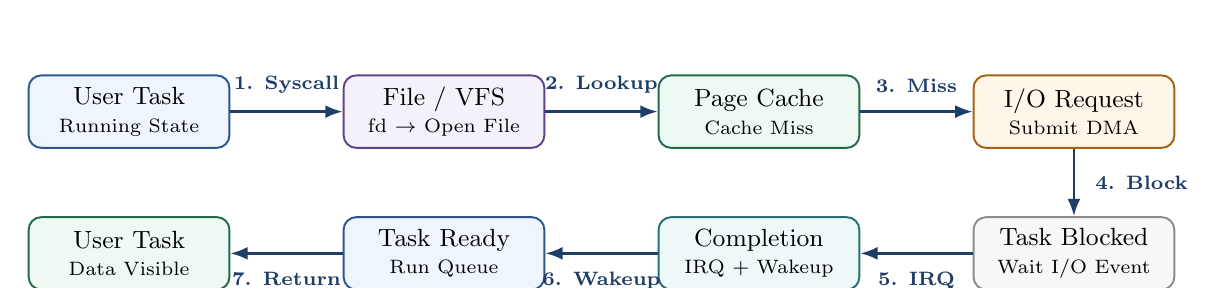
\begin{tikzpicture}[x=4.00cm,y=1.80cm]
  \node[knode] (u) at (0,0) {User Task\\[-1pt]\scriptsize Running State};
  \node[knodep] (fs) at (1,0) {File / VFS\\[-1pt]\scriptsize fd $\to$ Open File};
  \node[knodeg] (pc) at (2,0) {Page Cache\\[-1pt]\scriptsize Cache Miss};
  \node[knodeo] (io) at (3,0) {I/O Request\\[-1pt]\scriptsize Submit DMA};
  \node[knodegray] (blk) at (3,-1) {Task Blocked\\[-1pt]\scriptsize Wait I/O Event};
  \node[knodet] (irq) at (2,-1) {Completion\\[-1pt]\scriptsize IRQ + Wakeup};
  \node[knode] (ready) at (1,-1) {Task Ready\\[-1pt]\scriptsize Run Queue};
  \node[knodeg] (ret) at (0,-1) {User Task\\[-1pt]\scriptsize Data Visible};

  \draw[mainflow] (u) -- node[above=3pt,font=\scriptsize\bfseries,text=deepblue]{1. Syscall} (fs);
  \draw[mainflow] (fs) -- node[above=3pt,font=\scriptsize\bfseries,text=deepblue]{2. Lookup} (pc);
  \draw[mainflow] (pc) -- node[above=3pt,font=\scriptsize\bfseries,text=deepblue]{3. Miss} (io);
  \draw[mainflow] (io) -- node[right=4pt,font=\scriptsize\bfseries,text=deepblue]{4. Block} (blk);
  \draw[mainflow] (blk) -- node[below=3pt,font=\scriptsize\bfseries,text=deepblue]{5. IRQ} (irq);
  \draw[mainflow] (irq) -- node[below=3pt,font=\scriptsize\bfseries,text=deepblue]{6. Wakeup} (ready);
  \draw[mainflow] (ready) -- node[below=3pt,font=\scriptsize\bfseries,text=deepblue]{7. Return} (ret);
\end{tikzpicture}
\end{center}

\begin{center}
\small
\begin{tabularx}{\linewidth}{>{\bfseries}p{0.18\linewidth} X}
\toprule
槽位 & 本题关键内容 \\
\midrule
Objects & task、fd table、open file、inode、page-cache page、I/O request、device \\
Relations & fd$\to$file$\to$inode；file/page-index$\to$page cache；request$\to$device \\
Queues & task I/O wait queue、run queue、device request queue \\
Events & syscall、cache miss、submit、block、DMA completion、interrupt、wakeup、dispatch \\
Mechanism & VFS lookup、block mapping、DMA、interrupt、sleep/wakeup、context switch \\
Policy & scheduler；若多个 I/O 请求则 request ordering \\
Invariant & user buffer 权限合法；request 只能正确完成一次；blocked/ready 状态一致 \\
Cost & page-cache hit 是 fast path；miss 进入 storage slow path；copy 与 I/O 是主要成本 \\
\bottomrule
\end{tabularx}
\end{center}

\section{第 15 章：母题三——file-backed mmap 的首次访问}

\[
\begin{aligned}
\code{mmap(file)}&\arr VMA\ created\arr first\ load/store\\
&\arr page\ fault\arr file\ page\ resolve\\
&\arr I/O?\arr PTE\ update\arr retry.
\end{aligned}
\]

\begin{center}
\small
\begin{tabularx}{\linewidth}{>{\bfseries}p{0.18\linewidth} X}
\toprule
槽位 & 本题关键内容 \\
\midrule
Objects & task、VMA、PTE、file/inode、page-cache page、physical frame \\
Relations & VA$\to$VMA；VMA$\to$file+offset；PTE$\to$frame；file page$\to$page cache \\
Queues & cache miss 时可能出现 I/O wait \\
Events & mmap syscall、first access、page fault、I/O completion \\
Mechanism & fault handling、file-backed page lookup、PTE install、instruction retry \\
Policy & frame allocation/reclaim 可能涉及选择；普通映射命中时无策略 \\
Invariant & 权限、文件映射范围、进程隔离正确 \\
Cost & lazy mapping 把实际 I/O 推迟到 first-touch slow path；后续访问回到 MMU fast path \\
\bottomrule
\end{tabularx}
\end{center}

\section{第 16 章：母题四——fork + COW + 文件描述符共享}

同一次 \code{fork()} 后，两类关系具有完全不同的语义：
\[
\boxed{Memory:\ separate\ logical\ address\ spaces\ +\ temporarily\ shared\ frames}
\]
\[
\boxed{File:\ separate\ fd\ tables\ +\ references\ to\ same\ open\ file\ description}
\]

因此 child 写内存时：
\[
COW\ fault\arr new\ frame\arr child\ PTE\ update,
\]
而父子对共享 OFD 的 \code{read/lseek} 可能共同改变同一个 offset。

\begin{exam}[跨专题识别点]
题目问“fork 以后是否共享”时禁止回答“共享/不共享”两个字。必须先问：\kw{共享的是哪个对象或哪条关系？} Address space identity、physical frame、fd table、open file description、inode 都不是同一层。
\end{exam}

\section{第 17 章：母题五——Mutex contention}

\[
T_1:acquire\rightarrow owner,
\]
\[
T_2:acquire\rightarrow atomic\ fail\rightarrow wait\ queue\rightarrow Blocked.
\]
随后：
\[
T_1:unlock\rightarrow wake(T_2)\rightarrow Ready\rightarrow scheduler\rightarrow Running.
\]

\begin{center}
\small
\begin{tabularx}{\linewidth}{>{\bfseries}p{0.18\linewidth} X}
\toprule
槽位 & 本题关键内容 \\
\midrule
Objects & T1、T2、mutex/lock object \\
Relations & owner relation：lock$\to$T1；waiter relation：T2$\to$lock \\
Queues & lock wait queue + run queue \\
Events & acquire、atomic failure、sleep、unlock、wakeup、dispatch \\
Mechanism & atomic RMW、sleep/wakeup、scheduler \\
Policy & 多个 waiter 时可能有公平/优先级选择 \\
Invariant & mutual exclusion；不能 lost wakeup；owner/lifetime 合法 \\
Cost & uncontended fast path vs contended block/schedule slow path \\
\bottomrule
\end{tabularx}
\end{center}

\section{第 18 章：母题六——Pipe empty/full 与背压}

Pipe 是非常纯粹的跨专题对象：它既是 fd 可引用的内核对象，又有 buffer state、reader/writer waiters 和 blocking semantics。

\[
Reader\ +\ Empty\ Pipe\arr Blocked,
\]
\[
Writer\ writes\arr BufferStateChange\arr WakeReader.
\]
反向：
\[
Writer\ +\ Full\ Pipe\arr Blocked,
\]
\[
Reader\ consumes\arr FreeSpace\arr WakeWriter.
\]

所谓 backpressure 不需要再成为独立 Law，它只是本题状态机中的结果：
\[
\boxed{Demand>BufferCapacity\Rightarrow Enqueue/Block.}
\]

\section{第 19 章：母题七——Memory Pressure 的一生}

\begin{center}
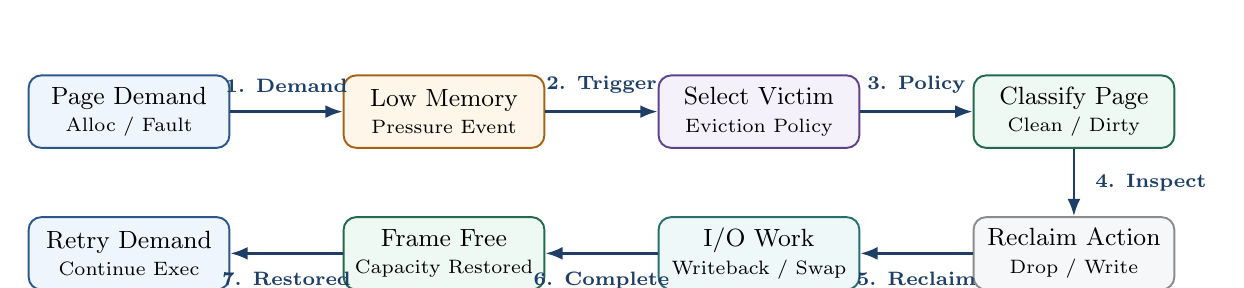
\begin{tikzpicture}[x=4.00cm,y=1.80cm]
  \node[knode] (req) at (0,0) {Page Demand\\[-1pt]\scriptsize Alloc / Fault};
  \node[knodeo] (press) at (1,0) {Low Memory\\[-1pt]\scriptsize Pressure Event};
  \node[knodep] (victim) at (2,0) {Select Victim\\[-1pt]\scriptsize Eviction Policy};
  \node[knodeg] (type) at (3,0) {Classify Page\\[-1pt]\scriptsize Clean / Dirty};
  \node[knodegray] (action) at (3,-1) {Reclaim Action\\[-1pt]\scriptsize Drop / Write};
  \node[knodet] (io) at (2,-1) {I/O Work\\[-1pt]\scriptsize Writeback / Swap};
  \node[knodeg] (free) at (1,-1) {Frame Free\\[-1pt]\scriptsize Capacity Restored};
  \node[knode] (retry) at (0,-1) {Retry Demand\\[-1pt]\scriptsize Continue Exec};

  \draw[mainflow] (req) -- node[above=3pt,font=\scriptsize\bfseries,text=deepblue]{1. Demand} (press);
  \draw[mainflow] (press) -- node[above=3pt,font=\scriptsize\bfseries,text=deepblue]{2. Trigger} (victim);
  \draw[mainflow] (victim) -- node[above=3pt,font=\scriptsize\bfseries,text=deepblue]{3. Policy} (type);
  \draw[mainflow] (type) -- node[right=4pt,font=\scriptsize\bfseries,text=deepblue]{4. Inspect} (action);
  \draw[mainflow] (action) -- node[below=3pt,font=\scriptsize\bfseries,text=deepblue]{5. Reclaim} (io);
  \draw[mainflow] (io) -- node[below=3pt,font=\scriptsize\bfseries,text=deepblue]{6. Complete} (free);
  \draw[mainflow] (free) -- node[below=3pt,font=\scriptsize\bfseries,text=deepblue]{7. Restored} (retry);
\end{tikzpicture}
\end{center}

这道母题把 VM、Page Cache、File System、I/O 与 Scheduling 接起来：
\begin{itemize}
  \item clean file-backed page：可丢弃，未来从文件恢复；
  \item dirty file-backed page：通常先 writeback，进入 I/O；
  \item anonymous page：若要回收，可能依赖 swap 或其他机制；
  \item 如果 reclaim/I/O 不能立即完成，当前 task 可能等待。
\end{itemize}

\begin{corebox}[最关键的分工]
\kw{Pressure} 是事件/状态条件；\kw{Victim selection} 是 Policy；\kw{unmap/writeback/swap/reclaim} 是 Mechanism；\kw{不能回收仍被必要引用或 pinned 的页}属于 Invariant；最终回收延迟和 I/O 是 Cost。
\end{corebox}

\section{第 20 章：母题八——write + fsync + crash}

必须区分四个状态：
\[
\boxed{UserBuffer\rightarrow PageCacheDirty\rightarrow DeviceCompleted\rightarrow DurableState}
\]
它们不是同一个“写完”。

\begin{center}
\small
\begin{tabularx}{\linewidth}{>{\bfseries}p{0.18\linewidth} X}
\toprule
槽位 & 本题关键内容 \\
\midrule
Objects & file/inode、dirty pages、journal transaction、block requests、device cache \\
Relations & file offset$\to$page cache；metadata$\to$journal/blocks \\
Queues & writeback/I/O request queue \\
Events & write、dirty threshold、fsync、I/O completion、crash、recovery \\
Mechanism & dirty marking、writeback、journal commit、flush/FUA/设备完成、replay \\
Policy & writeback timing / allocation / request scheduling 等可能存在策略 \\
Invariant & crash 后 metadata/namespace 必须可恢复到合法状态；fsync 语义必须满足 \\
Cost & 延迟写降低前台延迟，却把持久化成本推迟到 writeback/fsync slow path \\
\bottomrule
\end{tabularx}
\end{center}

\section{第 21 章：母题九——unlink while open}

\begin{center}
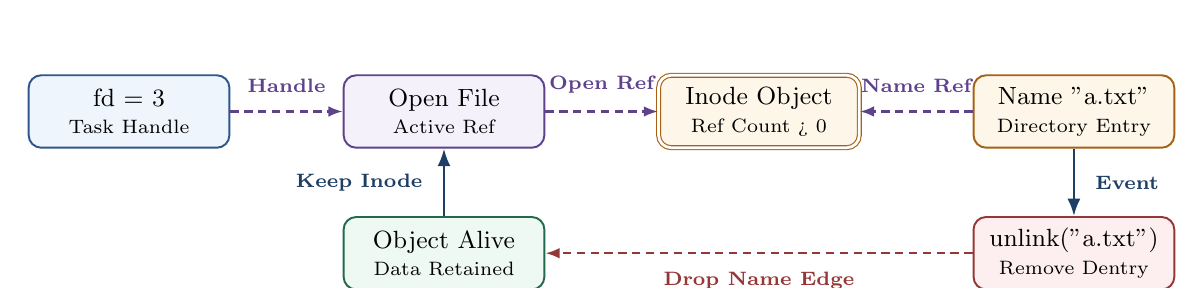
\begin{tikzpicture}[x=4.00cm,y=1.80cm]
  \node[knode] (fd) at (0,0) {fd = 3\\[-1pt]\scriptsize Task Handle};
  \node[knodep] (file) at (1,0) {Open File\\[-1pt]\scriptsize Active Ref};
  \node[persistent] (inode) at (2,0) {Inode Object\\[-1pt]\scriptsize Ref Count > 0};
  \node[knodeo] (name) at (3,0) {Name "a.txt"\\[-1pt]\scriptsize Directory Entry};

  \node[knodered] (unlink) at (3,-1) {unlink("a.txt")\\[-1pt]\scriptsize Remove Dentry};
  \node[knodeg] (alive) at (1,-1) {Object Alive\\[-1pt]\scriptsize Data Retained};

  \draw[relation] (fd) -- node[above=3pt,font=\scriptsize\bfseries,text=purple]{Handle} (file);
  \draw[relation] (file) -- node[above=3pt,font=\scriptsize\bfseries,text=purple]{Open Ref} (inode);
  \draw[relation] (name) -- node[above=3pt,font=\scriptsize\bfseries,text=purple]{Name Ref} (inode);
  \draw[mainflow] (name) -- node[right=4pt,font=\scriptsize\bfseries,text=deepblue]{Event} (unlink);
  \draw[danger,densely dashed] (unlink) -- node[below=3pt,font=\scriptsize\bfseries,text=deepred]{Drop Name Edge} (alive);
  \draw[mainflow] (alive) -- node[left=4pt,font=\scriptsize\bfseries,text=deepblue]{Keep Inode} (file);
\end{tikzpicture}
\end{center}

本题只要坚持 State 模型就不会错：\code{unlink()} 删除一条 Naming relation，不等于立刻从 Objects 集合删除 inode/file data。真正回收要等剩余引用关系满足生命周期不变量。

\newpage
\section{Part VI：408 综合题统一协议}

\section{第 22 章：跨专题十六问}

拿到综合题不要先回忆“这是哪一章”。按顺序问：
\begin{enumerate}
  \item 当前有哪些 \kw{Objects}？
  \item 当前各对象处于什么 \kw{State}？
  \item 有哪些 \kw{Relations/Mapping}？
  \item 是否存在 \kw{Queue/Waiter}？
  \item 当前真正发生了什么 \kw{Event}？
  \item CPU 此刻在 User 还是 Kernel？
  \item 哪个 \kw{Mechanism}允许这次状态转换？
  \item 是否存在多个合法候选动作？若有，哪个 \kw{Policy}选择？
  \item 哪条 \kw{Protection/Safety Invariant}必须保持？
  \item 是否涉及 \kw{Progress/Liveness}？谁能制造继续运行的事件？
  \item 是否涉及对象 \kw{Lifetime}？哪些引用被创建/删除？
  \item 数据此刻在哪里？是否在 cache/buffer/device 中移动？
  \item 是否发生 fast-path miss，进入 slow path？
  \item 如果 Demand$>$Capacity，谁排队、阻塞、回收或被拒绝？
  \item 如果中途 crash/interleaving，是否留下非法部分状态？
  \item 最终题目问的是哪个 Cost：时间、空间、I/O、公平、竞争还是持久性？
\end{enumerate}

\section{第 23 章：一页式综合决策树}

\begin{center}
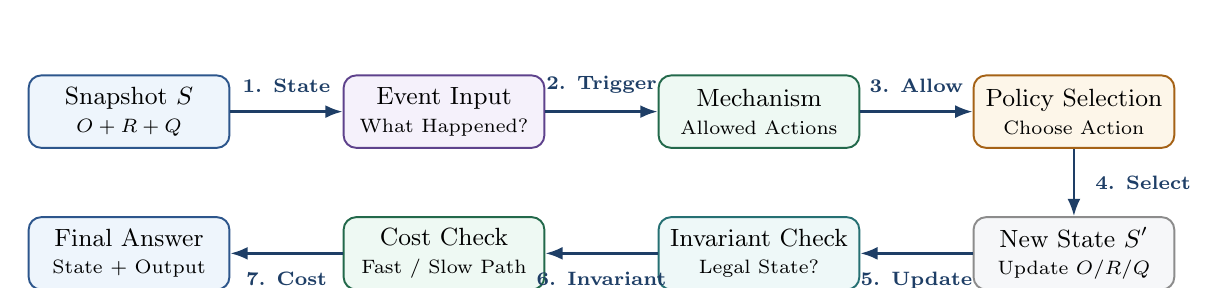
\begin{tikzpicture}[x=4.00cm,y=1.80cm]
  \node[knode] (s) at (0,0) {Snapshot $S$\\[-1pt]\scriptsize $O + R + Q$};
  \node[knodep] (e) at (1,0) {Event Input\\[-1pt]\scriptsize What Happened?};
  \node[knodeg] (m) at (2,0) {Mechanism\\[-1pt]\scriptsize Allowed Actions};
  \node[knodeo] (p) at (3,0) {Policy Selection\\[-1pt]\scriptsize Choose Action};
  \node[knodegray] (n) at (3,-1) {New State $S'$\\[-1pt]\scriptsize Update $O / R / Q$};
  \node[knodet] (i) at (2,-1) {Invariant Check\\[-1pt]\scriptsize Legal State?};
  \node[knodeg] (c) at (1,-1) {Cost Check\\[-1pt]\scriptsize Fast / Slow Path};
  \node[knode] (a) at (0,-1) {Final Answer\\[-1pt]\scriptsize State + Output};

  \draw[mainflow] (s) -- node[above=3pt,font=\scriptsize\bfseries,text=deepblue]{1. State} (e);
  \draw[mainflow] (e) -- node[above=3pt,font=\scriptsize\bfseries,text=deepblue]{2. Trigger} (m);
  \draw[mainflow] (m) -- node[above=3pt,font=\scriptsize\bfseries,text=deepblue]{3. Allow} (p);
  \draw[mainflow] (p) -- node[right=4pt,font=\scriptsize\bfseries,text=deepblue]{4. Select} (n);
  \draw[mainflow] (n) -- node[below=3pt,font=\scriptsize\bfseries,text=deepblue]{5. Update} (i);
  \draw[mainflow] (i) -- node[below=3pt,font=\scriptsize\bfseries,text=deepblue]{6. Invariant} (c);
  \draw[mainflow] (c) -- node[below=3pt,font=\scriptsize\bfseries,text=deepblue]{7. Cost} (a);
\end{tikzpicture}
\end{center}

\begin{corebox}[最终心智模型]
\[
\boxed{\text{Snapshot }S=(Objects,Relations,Queues)}
\]
\[
\boxed{\text{Event}\rightarrow\text{Mechanism}\rightarrow\text{Policy(if needed)}\rightarrow S'}
\]
\[
\boxed{Invariant(S')=true\quad\text{and}\quad Cost\text{ is acceptable}}
\]

所谓进程、虚拟内存、并发、I/O、文件系统，只是在改变：\kw{对象类型、关系类型、队列类型、事件类型、机制与策略、不变量和成本函数}。这就是本册唯一需要保留的统一语言。
\end{corebox}

\section{附录 A：概念去重检查表}

\begin{center}
\small
\begin{tabularx}{\linewidth}{>{\bfseries}p{0.24\linewidth} X X}
\toprule
概念 & 正式出现位置 & 遇到相关题时怎么用 \\
\midrule
Naming/Indirection & Relations & 画出逻辑名字/句柄到对象的边 \\
Protection/Isolation & Invariants & 检查“主体-操作-对象”是否允许 \\
Mechanism/Policy & Transition & 先列合法动作，再判断是否需要选择 \\
Scarcity/Arbitration & Queue + Policy & 先确认是否排队，再问策略选谁 \\
Backpressure & Queue 状态变化 & 供给不足时分析阻塞、排队、拒绝或回收 \\
Consistency/Recovery & Invariant + repair & 找出部分完成状态与修复路径 \\
Fast/Slow Path & Cost & 比较常见路径与 miss/conflict 的成本差 \\
Event-driven & Event & 找真正触发状态改变的输入 \\
Lifetime/Ownership & O/R 演化 + 约束 & 追踪引用增减与最终销毁条件 \\
Caching/Lazy/Batching & Cost optimization & 解释为何推迟、复用或合并工作 \\
\bottomrule
\end{tabularx}
\end{center}

\section{附录 B：专题到综合篇的边界}

\begin{itemize}
  \item \kw{进程专题}负责讲清 task/process/thread、调度算法、trap/context switch 的局部机制；综合篇只追踪它们怎样与其他对象共同变化。
  \item \kw{并发/PV 专题}负责同步原语和经典模型；综合篇只抽象为 lock object、wait queue、event、invariant。
  \item \kw{虚拟内存专题}负责页表、TLB、fault 与 replacement；综合篇只追踪 VM 事件怎样继续进入文件、I/O 与进程状态。
  \item \kw{I/O 专题}负责 polling、interrupt、DMA、driver、page cache 与 spooling；综合篇只追踪 request、block、completion 与 wake。
  \item \kw{文件系统专题}负责 path/fd/inode/block/journal；综合篇只关注这些关系怎样跨 VM/I/O/进程状态传播。
\end{itemize}

\begin{method}[本册的唯一功能]
专题册负责“把一个机制打穿”；综合册负责“让多个已经学会的机制在同一状态机里同时运行”。因此本册不再重复定义页表、PV、inode 或 DMA，而只训练跨对象、跨事件、跨不变量的推演。
\end{method}

\end{document}
